\begin{frame}
\frametitle{Кооперативная многозадачность}
\begin{itemize}
   \item<1->Невытесняющая (кооперативная) многозадачность
   \begin{itemize}
      \item<1->поток должен сам вызвать функцию переключения;
      \item<2->что если в коде содержится ошибка?
      \item<3->или мы обращаемся к библиотеке, которая выполняет долгую операцию?
   \end{itemize}
\end{itemize}
\end{frame}

\begin{frame}
\frametitle{Вытесняющая многозадачность}
\begin{itemize}
    \item<1->Вытесняющая (preemptive) многозадачность
    \begin{itemize}
        \item<1->поток снимается ОС с CPU "силой", по истечению \emph{кванта}
             времени;
        \item<2->синхронизация потоков при этом усложняется;
        \item<3->как организовать вытесняющую многозадачность?
    \end{itemize}
\end{itemize}
\end{frame}

\begin{frame}
\frametitle{Сново о прерываниях}
\begin{itemize}
    \item<1->Обработчик прерывания "прерывает" исполняемый код
    \begin{itemize}
        \item<2->но обработчик работает в контексте прерванного потока;
        \item<3->функцию переключения контекста можно вызвать от имени потока
             из обработчика прерываний.
    \end{itemize}
\end{itemize}
\end{frame}

\begin{frame}
\frametitle{Вытесняющая многозадачность}
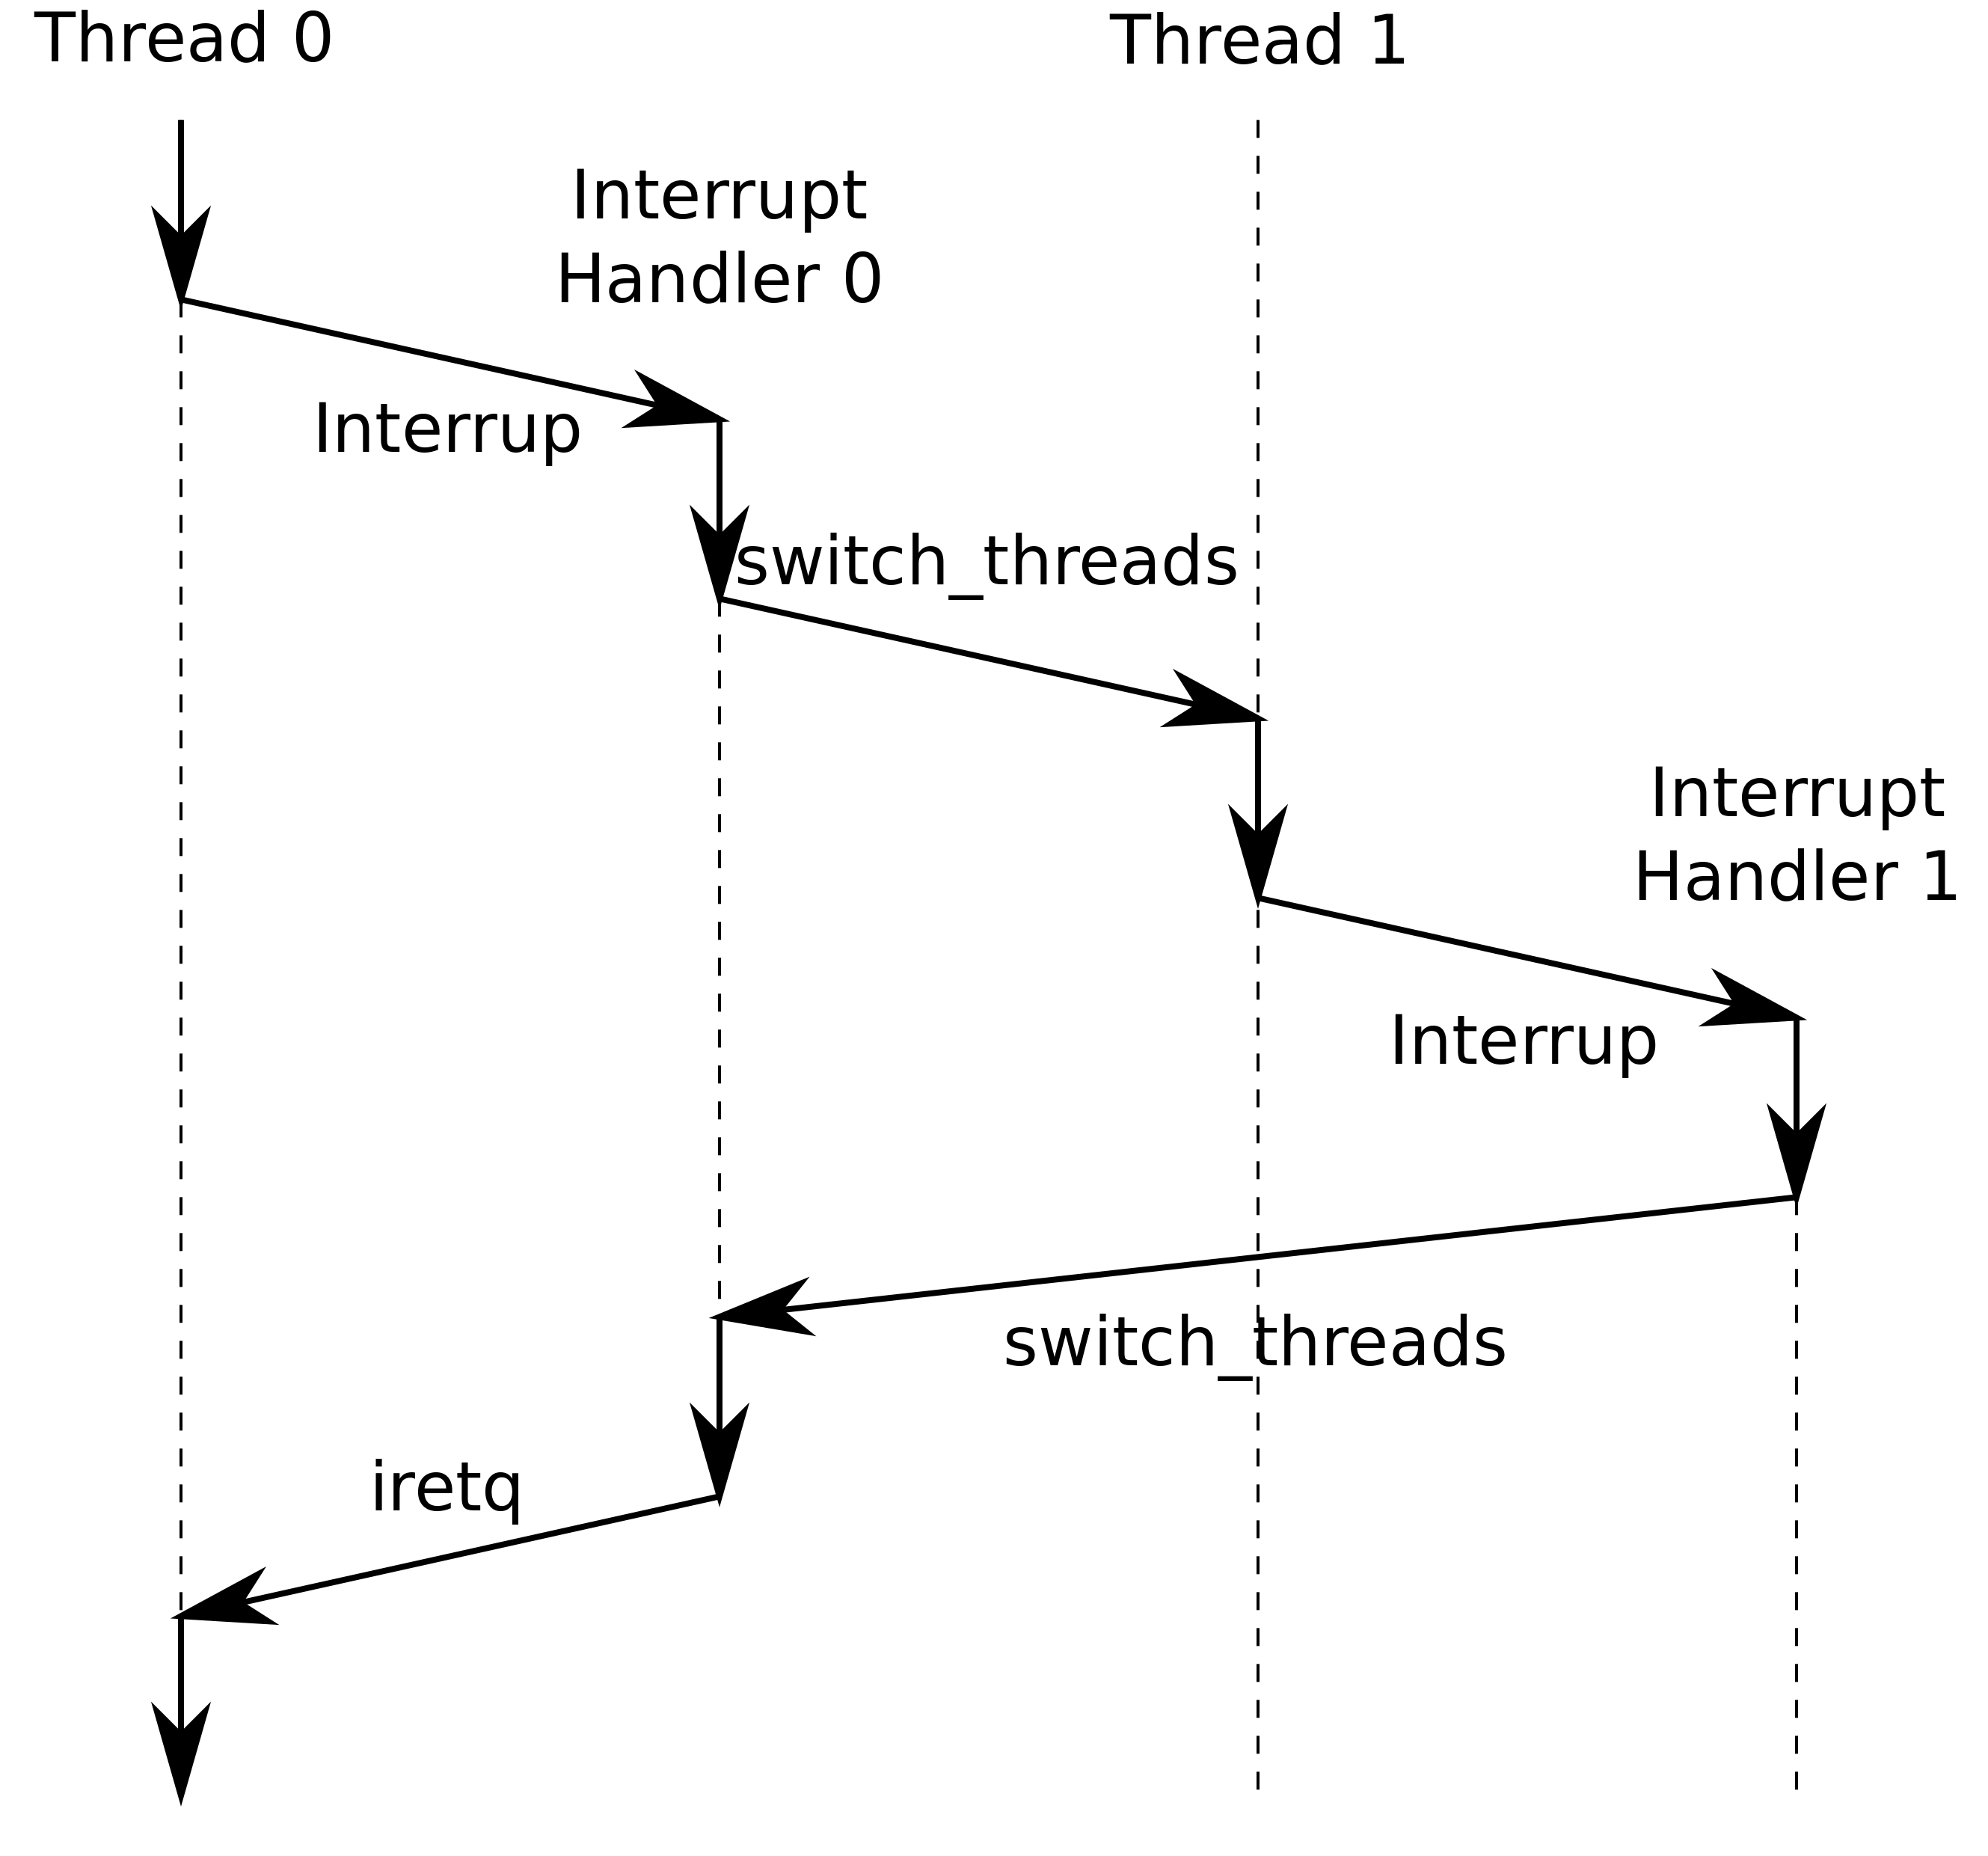
\includegraphics[height=.6\textheight]{preempt}
\end{frame}

\begin{frame}
\frametitle{Таймер}
\begin{itemize}
    \item<1->Таймер может генерировать прерывания с заданной периодичностью
    \begin{itemize}
        \item<1->Programmable Interval Timer (PIT, intel 8253) - IBM PC;
        \item<2->High Precision Event Timer (HPET);
        \item<3->Local APIC Timer.
    \end{itemize}
\end{itemize}
\end{frame}
